% !TEX root = ../Robotik.tex
\chapter{Navigation}
\section{Bekanntes vs. unbekanntes Terrain}
Man unterscheidet zwischen Algorithmen für:
\begin{itemize}
	\item \textbf{bekannte Umgebung:} auch während der Fahrt ändert sich die
		Umgebung nicht
	\item \textbf{unbekannte Umgebung:} entweder vollständig oder Teilweise
		unbekannte Umgebung
\end{itemize}

Ist das Gebiet \textbf{vollständig bekannt}, lässt sich die Suche mittels eines
Graphen lösen. Ansonsten erfolgen die Berechnungen auf lokalen
Teilinformationen von Sensoren mit denen \textbf{inkrementelle Anpassungen}
vorgenommen werden.

\section{Navigation in unbekanntem Terrain}
\subsection{Konturverfolgung}
Eine \textbf{Freiraumfahrt} d.h. eine Fahrt durch ein Gelände, dessen
Raum möglichst weit und frei von Hindernissen ist, ist nicht immer Zielführend.

Lösung: \textbf{Konturverfolgung}
\begin{itemize}
	\item Roboter wird nah an einem Objekt (Wand, Hinderniss) entlang bewegt
	\item Es sollte möglichst ein gegebener Abstand $d$ eingehalten werden
\end{itemize}

\begin{lstlisting}[language=bash, caption={Regelung des Abstands $d$}]
if (Distance to Wall > d) then
	turn to wall
fi

if (Distance to Wall < d) then
	turn away from wall
fi

if (Distance to Wall == d) then
	Drive straight ahead
fi
\end{lstlisting}

\pagebreak
\subsection{Bug1 Algorithmus}
{
\begin{wrapfigure}{r}{0.4\textwidth}
	\vspace{-1cm}
	\includegraphics[width=0.4\textwidth]{Resources/PNG/Bug1.PNG}
	\caption{Bug1 Algorithmus Route}
	\label{fig:PNG/Bug1.png}
\end{wrapfigure}
\paragraph{Vorraussetzungen}
\begin{itemize}
	\item Bewegung auf einer geraden Linie
	\item Konturverfolgung
	\item Roboter benötigt einen Sensor zur Erkennung eines "Kontakts" mit einem
		Hindernis
	\item Roboter kann die Distanz zwischen zwei Punkten x und y messen
	\item der Arbeitsraum ist begrenzt
\end{itemize}

}

\paragraph{Algorithmus}
\begin{lstlisting}[language=c++, caption={}]
while ( noch nicht am Ziel ) {
	try {
		Folge gerader Linie zum Ziel
	} catch ( HindernisKontakt kontaktpunkt ) {
		Umfahre das Hindernis bis wieder bei $kontaktpunkt
		leavepoint = Punkt mit Lot vom Hindernis zum Ziel
		Fahre zu $leavepoint
	}
}
\end{lstlisting}

\paragraph{Exception}
Schneidet die Linie von $q1^L$ zum Ziel das \textbf{aktuelle Hindernis} gibt
es keine Lösung
\begin{figure}[H]
	\begin{center}
		\includegraphics[scale=0.4]{Resources/PNG/Exception1.PNG}
		\caption{}
		\label{fig:PNG/Exception1.PNG}
	\end{center}
\end{figure}

\subsection{Bug2-Algorithmus}
Schnellere Variante zu Bug1, da Hindernis nicht komplett umrundet wird.
Eventuell keine mögliche Lösung wie bei Bug1. \textbf{Backtracking} und
damit Veränderung der Umfahrichtung eines Hindernisses können helfen.

\pagebreak

\begin{lstlisting}[language=c++, caption={Algorthmus ohne Backtracking}]
/**
 * Start S
 * Ziel T
 * Derzeitige Position P = S
 * Umfahrrichtung = rechts
 */
Konstruiere Strecke ST
while (nicht bei T) {
	try {
		Fahre auf ST
	} catch (HindernisKontaktPunkt H) {
		while (P == Schnittpunkt mit ST && len(PT) < len(HT)) {
			Umfahre das Objekt rechtsherum
		}
	}
}
\end{lstlisting}

\subsection{Bug3-Algorithmus}
Unterschied zu Bug2 ist, dass er nicht der Strecke ST strikt folgt sondern
jede Möglichkeit nutzt näher ans Ziel T zu kommen. Auch hier Problematik keine
Lösung zu finden und Verbesserung durch Backtracking möglich.

\begin{lstlisting}[language=c++, caption={Algorthmus ohne Backtracking}]
/**
 * Start S
 * Ziel T
 * Derzeitige Position P = S
 * Umfahrrichtung = rechts
 */
while (nicht bei T) {
	try {
		Fahre zu T
	} catch (HindernisKontakt) {
		while (PT nicht frei) {
			Umfahre das Objekt rechtsherum
		}
	}
}
\end{lstlisting}

\subsection{Labyrinthe}
\subsubsection{Grundprobleme}
\begin{itemize}
	\item Es wird davon ausgeangen, dass der Roboter berühren oder "sehen" kann
	\item Zwei grundlegend Hauptprobleme:
		\begin{itemize}
			\item Einen \textbf{Weg in ein Labyrinth} finden, um einen bestimmten
				Gegenstand oder \textbf{Schatz zu erreichen} sowie den \textbf{Rückweg
				zum Eingang}
			\item \textbf{Flucht aus einem Labyrinth} von einer unbekannten Stelle
				aus.
		\end{itemize}
	\item Enger Zusammenhang zwischen Labyrinth und Graphen $\Rightarrow$ Jeder
		Korridor:= Kante und jede Kreuzung:= Knoten
	\subitem Bei bekanntem Labyrinthe $\Rightarrow$ Suchproblem in Bäumen
\end{itemize}

\subsubsection{Verlassen eines Labyrinths mit Pledge Algorithmus}
\textbf{Grundidee} Vorsichtig geradeaus bis man auf ein Hindernis trifft und
dann mit der "linken" Hand immer an der Wand entlang bis zum Ausgang.

\textbf{Problem} Enthält das Labyrinth eine Säule, läuft man für immer im
Kreis

\textbf{Lösung} Man folgt der Wand nur solange, bis man wieder in die alte
Richtung schaut.

\textbf{Allgemeingültige Lösung} Drehungen beim Abbiegen an den Ecken
mitzählen. Bei jeder Linksdrehung wird der Umdrehungszähler inkrementiert, bei
jeder Rechtsdrehung dekrementiert.
\begin{itemize}
	\item Bewege den Roboter geradeaus bis eine Wand erreicht ist
	\item Folge der Wand bis Umdrehungszähler 0 ist
\end{itemize}

\subsubsection{Verlassen eines Labyrinths mit Ariadenfaden}
\textbf{Ziel}: einen Weg zu einem versteckten Ziel im Labyrinth sowie wieder
zurück zum Eingang finden ohne dass eine Karte des Labyrinths bekannt ist

\textbf{Idee}: Wenn man ein Labyrinth betritt Faden ausrollen $\Rightarrow$
zurückverfolgen bringt einen zurück zum Eingang.

\textbf{Vorraussetzungen und grundsätzliches Vorgehen}
\begin{itemize}
	\item einer Wand folgen
	\item Umdrehen
	\item Kreuzungen erkennen
	\item Ziel erkennen
	\item Faden auslegen und wieder einsammeln
	\item Faden am Boden erkennen
	\item Faden zur nächsten Kreuzung folgen
\end{itemize}

\subsubsection{Tarry und Tremaux Algorthmus}
\begin{itemize}
	\item Beispiel für klassische Tiefensuche
	\item Richtung, in der sich das zu suchende Objekt befindet ist unbekannt.
	\item Graph kann zyklen enthalten
	\item Es wird ein zyklisch gerichteter Graph durch jede Kante konstruiert,
		wobei jede Kante nur einmal pro Richtung besucht wird
\end{itemize}

\textbf{Algorithmus:}
\begin{itemize}
	\item Starte willkürlich an einem Knoten
	\item Folge einem möglichen Pfad, markiere die Kante, in welcher Richtung
		sie betreten worden ist
	\item Sind alle Kanten schon betreten, eine auswählen, die bis jetzt nur in
		die Gegenrichtung betreten wurde.
	\item Trifft man auf eine Sackgasse oder einen schon besuchten Gang, zurück
		zur letzten Kreuzung
	\item Es darf kein Pfad betreten werden, der schon in beide Richtungen
		besucht wurde.
	\item Algorithmus ist beendet, wenn der Startpunkt erreicht wird.
\end{itemize}

\section{Pfadplanung für mobile Roboter in bekanntem Terrain}
Ziel der Navigation ist es, ein Fahrzeug in der Umwelt zu bewegen.
Dies beinhaltet drei Unteraufgaben:
\begin{description}
	\item[Global Pfadplanung]
	\begin{itemize}
		\item \textbf{Vorraussetzung}: es gibt eine Karte
		\item suche eines Pfades von einem Start- zu einem Zielpunkt in vorhandenem Umgebungsmodell
		\item evtl. auch Suche nach Pfad mit geringsten Kosten
		\item Kompletter Pfad beschrieben durch Menge von Punkten
	\end{itemize}
	\item[Lokale Pfadplanung] berücksichtigt Fahrzeug-Dimension und kinematische
		Einschränkungen
	\item[Path Control] generiert geeignet Steuerbefehle, um den vorberechneten
		Pfad zu folgen
\end{description}

\subsection{Konfigurationsraum}
Summe aller Konfigurations-Hindernisse bildet den \textbf{Konfigurationsraum}.
Dieser ist eine Datenstruktur, die es dem Roboter ermöglicht, die \textbf{
Position und Orientierung von Hindernissen} in der Umgebung zu definieren. Der
Konfiguration dient somit als \textbf{Basis der Webplanung}.

\paragraph{Herleitung}
\begin{itemize}
	\item Abmesungen, Form, Bewegungsmöglichkeiten des Roboters werden für die
		Erstellung des Konfigurationsraums benötigt
	\item Konfiguration $q$ eines Roboters beschreibt Lage und Ausrichtung im
		Bezugssystem des Umgebungsmodells
	\item Im zweidimensionalen Raum kann Position in $x,y$-Ebene und Orientierung
		ausgedrückt werden
	\item Konstruktionsbedingt sind einige Konfigurationen für den Roboter in
		seiner Umgebung nicht zulässig
	\item Problem; einfachere Darstellung:
	\subitem Roboter als Punkt angenommen
	\subitem Abmessungen des Roboters + Objektabmessungen $\Rightarrow$
		Konfigurations-Hindernisse
\end{itemize}
\begin{figure}[H]
	\begin{center}
		\includegraphics[scale=0.5]{Resources/PNG/KonfigurationsHindernisse.PNG}
		\caption{}
		\label{fig:PNG/KonfigurationsHindernisse.PNG}
	\end{center}
\end{figure}

\paragraph{Repräsentationen}
\begin{itemize}
	\item Graphen mit Knoten
	\item Reguläre Gitter
	\item Quad-Bäume oder Octal-Bäume
	\item Voronoidiagramme
\end{itemize}

\section{Algorithmen und Methoden}
Für die folgenden Algorithmen und Methoden wird ausgeganen, dass Hindernisse
bekannt sind und weder Position noch Form ändern.

\paragraph{Zellzerlegungen} Das Umgebungsmodell wird in sich nicht überlappende
Zellen unterteilt, die als besetzt oder frei markiert sind

\paragraph{Straßenkartenmethoden oder Roadmaps}
Eine Roadmap ist ein Graph mit Knoten und Kanten, bei dem alle befahrbaren
Wege hinterlegt sind. Daraus kann ein kollisionsfreier Pfad vom Start- zum
Zielpunkt erstellt werden.

Auf dieses Netzwerk können Standardmethoden der Graphentheorie, wie sie auch in
der Autonavigation Verwendung finden, andwendet werden:
\begin{itemize}
	\item kürzeste Wegsuche mit A*, Dijkstra
	\item Wegsuche mit Umgehung von Hindernissen mit dem
		\textbf{Sichtbarkeitsgraph}
	\item Wegsuche mittels eines \textbf{Voronoigraphen},
		\textbf{Voronoidiagramms}
\end{itemize}

\paragraph{Potentialfeldmethoden} beinhalten die physikalische Simulation des
Roboters als Partikel in einem Feld.

\subsection{Dijkstra}
\begin{lstlisting}[language=c++]
/**
 * PriorityQueue Open
 */
struct Knoten {
	int cost
	Knoten* predecessor
}
Knoten start = {0, null};
push start on Open

while (Open is not empty) {
	Knoten n = pop lowest cost from Open
	if (ist n Ziel?) {
		konstruiere weg
		return sucess
	}
	for (Knoten nx : nachfolger von n) {
		newcost = n.cost + wegkosten von n nach nx
		if (n ist in Open && nx.cost <= newcost) {
			continue;
		}
		nx.predecessor = n
		nx.cost = newcost
		if (nx is not in Open) {
			push nx in Open
		}
	}
}
return failure
\end{lstlisting}

\subsection{A*}
\begin{lstlisting}[language=c++]
/**
 * PriorityQueue Open
 * List Closed
 */
struct Knoten {
	int total 					// total cost
	int est							// estimated cost
	int known 					// known cost
	Knoten* predecessor
}
Knoten start;
start.total = 0;
start.est = GoalDistEstimate(start);
start.known = start.total + start.est;
start.predecessor = null;

push start on Open

while (Open is not empty) {
	Knoten n = pop lowest total cost from Open
	if (ist n Ziel?) {
		konstruiere weg
		return sucess
	}
	for (Knoten nx : nachfolger von n) {
		newcost = n.known + wegkosten von n nach nx
		if ((n ist in Open || n ist in Closed) && nx.known <= newcost) {
			continue;
		}
		nx.predecessor = n
		nx.known = newcost
		nx.est = GoalDistEstimate(nx)
		nx.total = nx.known + nx.est
		if (nx is in Closed) {
			remove nx from Closed
		}
		if (nx is not in Open) {
			push nx in Open
		}
	}
	push n onto Closed
}
return failure
\end{lstlisting}

\subsection{Wegsuche mit dem Sichtgraph-Algorithmus}
\begin{description}
	\item[Visibility Map] Die Eckpunkte der Polygone (Hindernisse) werden zu
		Knoten, die eine Kante teilen wenn sie das Polygon nicht schneiden.
	\item[Visibility Graph] Einfachste Visibility Map, bei der Start- und
		Zielknoten mitinbegriffen sind. \textbf{Hinderniskanten sind Teil des
		Sichtgraphen}.
\end{description}

\subsubsection{Sichtgraphalgorithmus}
\begin{enumerate}
	\item Erzeuge Visiblity Graph $\Rightarrow$ Kanten = Wegstücke \& Knoten =
		Orte
	\item Kanten werden mit Entfernung gewichtet.
	\item Suche: Suche die Geraden, die den kürzesten Weg zum Ziel verbinden.
\end{enumerate}
Nachteile:
\begin{itemize}
	\item Weg tangiert Hindernisse
	\item Graph enthält viele nutzlose Kanten
\end{itemize}

\pagebreak
\subsubsection{Reduzierter Visibility Graph}
{
\begin{wrapfigure}{r}{0.4\textwidth}
	\includegraphics[width=0.4\textwidth]{Resources/PNG/SichtGraphReduziert}
\end{wrapfigure}
Der reduzierte Sichtgraph besteht nur aus unterstützenden und trennenden Kanten.
\begin{description}
	\item[unterstützende Kanten:] Tangente zu zwei Hindernis\-sen, so dass die
		Hindernisse auf derselben Seite der Linie liegen
	\item[trennende Kanten:] Tangente zu zwei Hindernissen so, dass die Hindernisse
		auf gegenüberliegenden Seiten der Tangente liegen.
\end{description}

Konstruktion:
Alle Liniensegmente $vv_i$ mit $v \neq v_i$ dürfen keinen Schnittpunkt mit
einer Hinderniskante haben.

$\Rightarrow$ \textbf{Nachteil:} Komplexität $O(n^3)$

$\Rightarrow$ \textbf{Effizienter:} Plane Sweep Algorithmus $O(n^2 log n)$

}
{
\begin{wrapfigure}{r}{0.4\textwidth}
	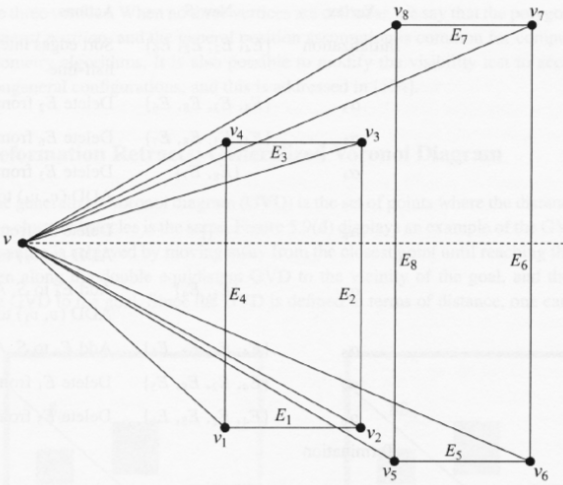
\includegraphics[width=0.4\textwidth]{Resources/PNG/sweepLineAlgorithmus}
\end{wrapfigure}
\ActivateWarningFilters[wrapfiglisting]
\begin{lstlisting}[language=c, caption={Sweep Line Algorithmus}]
/**
 * Input: Set of vertices (whose edges do not
 *         intersect) and a vertex v
 * Output: A subset of vertices from the
 *         input set that are within the line
 *         of sight of v
 */
Angles = vertices.map(vi ->
		angle between segment vvi horizontal line
		from v
)

Angles.sort(ASC)

List S // containing edges that intersect the
        // horizontal line from v

for (angle : Angles) {
	if (vi is visible to v)  {
		add edge (v, vi) to the visibility graph
	}
	if (vi ist the beginning of an edge, E, not in S) {
		insert E into S
	}
	if (vi is the end of and edge in S) {
		delete the edge form S
	}
}
\end{lstlisting}
\DeactivateWarningFilters[wrapfiglisting]

}

\pagebreak
\subsection{Voronoi-Diagramme}
{
\begin{wrapfigure}{r}{0.4\textwidth}
	\includegraphics[width=0.4\textwidth]{Resources/PNG/Polygon.PNG}
\end{wrapfigure}

Eine Fläche wird willkürlich mit Punkten besetzt. Diese Punkte bilden die
Zentren der Polygonflächen. Jeder Punkt der Fläche gehört zu dem Zentrum das
ihm am nächsten liegt $\Rightarrow$ Gehört zur Polygonfläche dieses Zentrums.
Wenn ein Punkt zu min. 2 Zentren den selben Abstand hat bildet er die Grenze
zwischen den Polygonflächen dieser Zentren. Der Abstand wird mit der
Euklidischen Abstandsfunktion bestimmt:
$$
	dist(p,q) = \sqrt{(p_x - q_x)^2 + (p_y - q_y)^2}
$$
Die Menge der Grenzlinien nennt man Voronoi-Diagramm

}

Immer dann gut einsetzbar, wenn ungenaue Sensoren zur Verfügung stehen oder die
Umwelt ungenau geometrisch modelliert wurde oder sich dynamisch ändert.

\subsubsection{Generalisierte Voronoi-Diagramme}
{
\begin{wrapfigure}{r}{0.4\textwidth}
	\vspace{-1cm}
	\centering
	\includegraphics[width=0.3\textwidth]{Resources/PNG/Voronoi.PNG}
\end{wrapfigure}
Bei dem sogenannten generalisierten Voronoi Diagramm (GVD) ist die \textbf{
Form der Zentren} und die Art der \textbf{Abstandsfunktion} nicht festgelegt.
Dadurch können Zentren komplexere Formen statt nur Punkte sein. Die damit
entstehenden Voronoi-Kanten bilden mögliche kollisionsfreie Wegstücke.

In der Robotik werden Konfigurationsräume gerne damit repräsentiert und die
Hindernisse werden zu Zentren des GVD gemacht. Bei der Wegfindung befinden sich
Start- und Zeilpunkt nicht auf dem Diagramm, diese werden mit der
nächstgelegenen Kante verbunden.

}

\subsection{Navigation in einer Rasterkarte}
{
\begin{wrapfigure}{r}{0.4\textwidth}
	\includegraphics[width=0.4\textwidth]{Resources/PNG/RasterKarte.png}
\end{wrapfigure}
In einer Rasterkarte gibt es nur die Bewegunsrichtungen (N, O, S, W). Sie
besteht aus einem binären Raster. Es können zwei ähnliche Algorithmen zur
Navigation verwendet werden:
\begin{itemize}
	\item Fluten vom Startpunkt aus
	\item Fluten vom Zielpunkt aus (Wave Front Planer)
\end{itemize}
Bei beiden Algorithmen werden in jeder Iteration die Werte des Nachbarn des
Randes der Welle, die kein Hindernis darstellen, auf den Wellenwert + 1 gesetzt.

Daraufhin kann der gewünschte Weg durch Absteigen (Backtracking) ermittelt
werden. Die beiden Algorthmen unterschieden sich in der Startbelegung.

}

\begin{table}
\centering
\begin{tabular}{r|l|l}
							  & \textbf{Fluten vom Startpunkt} & \textbf{Wave Front Planer} \\
\hline
Start der Welle & Startpunkt                     & Zielpunkt                  \\
Hindernis Wert  & -1                             & 1                          \\
Frei Startwert  & 0                              & 0                          \\
Wellen Startwert& 1                              & 2                          \\
Anmerkung       &                                & Einfache Potentialfeldmethode
\end{tabular}
\end{table}

\paragraph{Nachteile}
\begin{itemize}
	\item Weg fürht ev. nah am Hindernis vorbei
	\item Der gesamte Raum muss durchsucht werden
\end{itemize}

\paragraph{Vorteil} auch im 3D Raum anwendbar mit 6 Nachbarfeldern.

\begin{figure}[H]
	\begin{center}
		\includegraphics[]{Resources/PNG/Flooding.PNG}
		\caption{Flooding Algorithmus}
		\label{fig:PNG/Flooding.PNG}
	\end{center}
\end{figure}

\subsection{Potentialfeld Methode}
Vorbild ist das elektrische Feld. Dabei müssen Start- und Zielposition und die
Positionen aller Hindernisse bekannt sein. Der Zielpunkt und Freiraum erhalten
ein anziehendes Potential. Der Startpunkt, Hindernisse und Wände ein abstoßendes
Potential. Eine Karte mit den verschiedenen anziehenden und abstoßenden Kräften
wird erstellt, diese nehmen linear mit dem Abstand zum Objekt ab.

Der Roboter bewegt sich nach der Methode des steilsten Abstiegs im Potentialfeld
auf das Ziel zu.

\textbf{Problem} Der steile Abstieg ist ein greedy Algorthmus und kann dazu
führen, dass ein lokales Minima erreicht wird und somit in einer Sackgasse
landet. $\Rightarrow$ Potentialfunktion wählen, dass es nur ein Minima im Ziel
gibt.
